% Note from Eric Y: this is my preferred background section. We can decide which one to ultimately include later.

\documentclass[25pt,margin=1in,innermargin=-6.5in,blockverticalspace=0in]{tikzposter}
\geometry{paperwidth=48in,paperheight=36in,showframe}
\usepackage[utf8]{inputenc}
\usepackage{amsmath}
\usepackage{amsfonts}
\usepackage{amsthm}
\usepackage{amssymb}
\usepackage{graphicx}
\usepackage{adjustbox}
\usepackage{enumitem}
\usepackage{xcolor}
\usepackage[backend=biber,style=numeric]{biblatex}
\usepackage{emory-theme}
\usepackage{lmodern}




\renewcommand{\familydefault}{\sfdefault}
\usepackage{sansmath}
\sansmath

\usepackage{mwe} % for placeholder images

\addbibresource{frog.bib}

\newcommand{\edit}[1]{\textcolor{red}{#1}}

% set theme parameters
\tikzposterlatexaffectionproofoff
\usetheme{EmoryTheme}
\usecolorstyle{EmoryStyle}

\title{Monotonicity for the Frog Model with Drift on Trees}
\author{Yanni Bills, Feng Cheng, Eric Han, Viet Le, Scott Wynn, Eric Yu}
\institute{Polymath Jr.\ (Poster No.\ 106)}
\titlegraphic{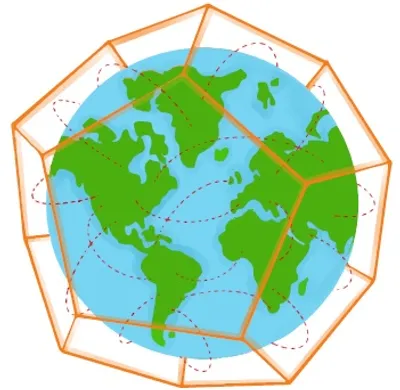
\includegraphics[width=0.065\textwidth]{Polylogo.png}}

% begin document
\begin{document}

\maketitle
\centering
\begin{columns}

\column{0.25}
\block{Abstract}{
    \fontsize{37}{45} \selectfont The frog model with drift starts with an active particle at the root of the infinite $d$-ary tree and dormant particles at each non-root site. In discrete time, active particles move towards the root with probability $p$, and otherwise move to a uniformly sampled child vertex. When an active particle moves to a site containing dormant particles, all the particles at the site become active. The critical drift $p_d$ is the infimum over all $p$ for which infinitely many particles visit the root almost surely. We have improved bounds on $\sup_{d\geq m}p_d$ and proved monotonicity of critical values associated to a self-similar variant.
    \begin{tikzfigure}[frog model on the $2$-ary tree]
        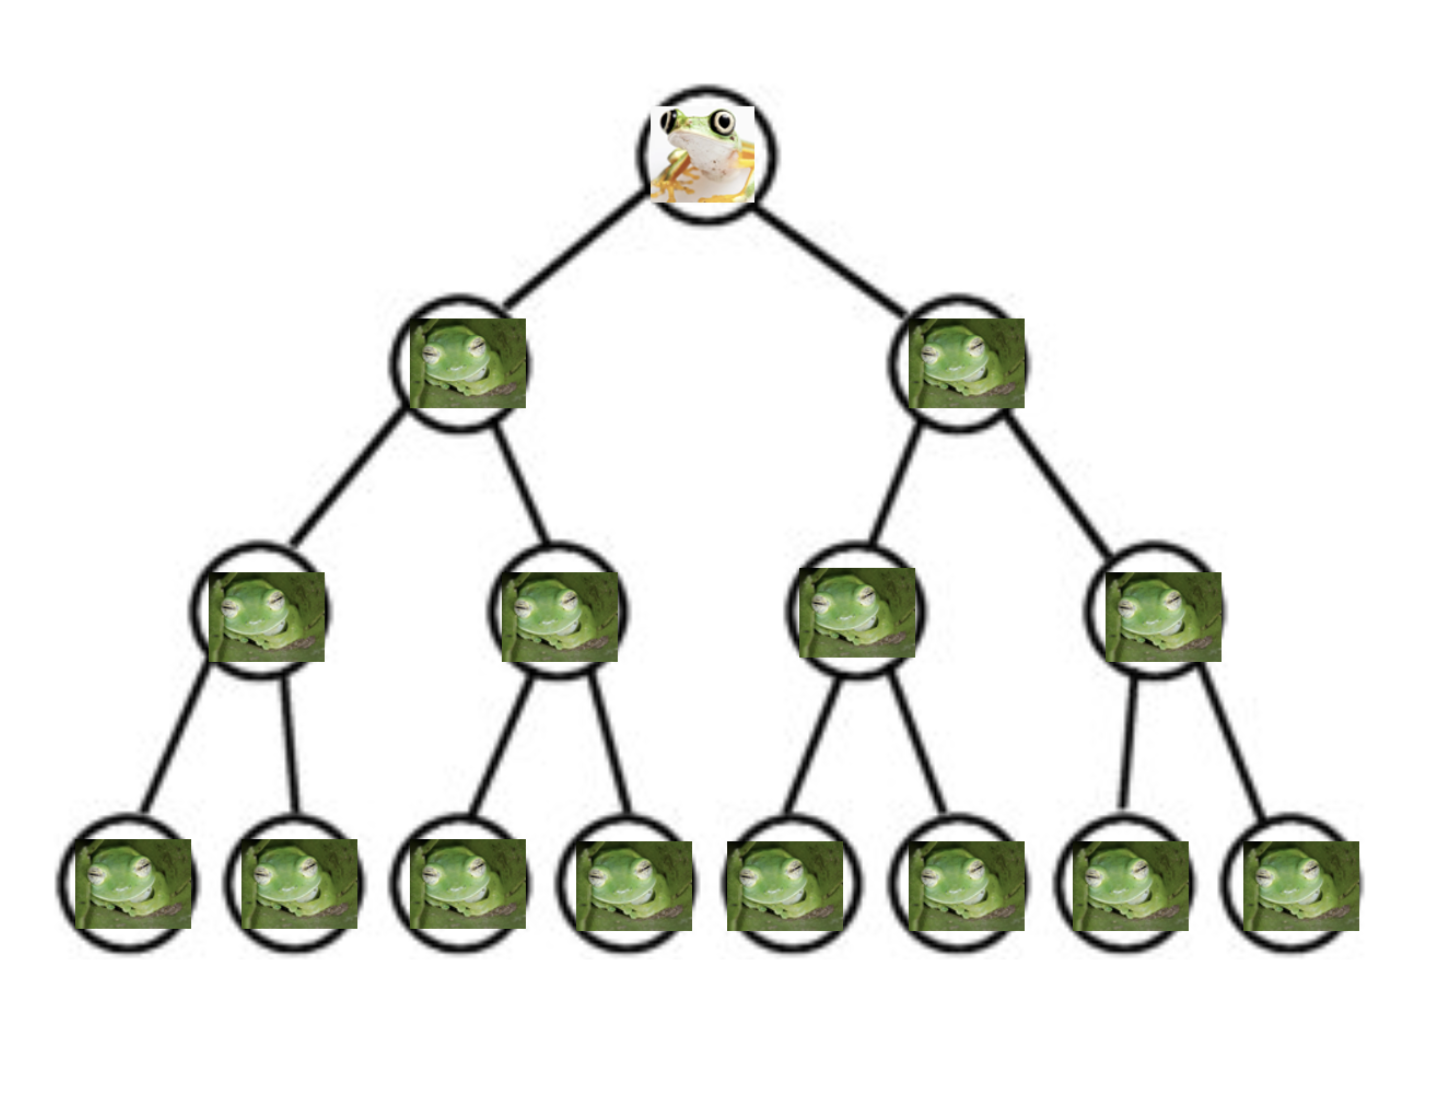
\includegraphics[width=0.5\linewidth]{tree.png}
    \end{tikzfigure}
}

\block{Background}{
    The frog model can be viewed as a model of combustion, rumor spread, infection, etc. The behavior of frogs on the integer lattice $\mathbf{Z}^d$ is well-studied, but their behavior on trees has remained a difficult question.

    

    %  \vspace{0.5 cm}
     
    %  \textbf{Things we know:}
    %  \begin{itemize}
    %      \item $p_1 = \frac{1}{2} = 0.5$
    %      \item $p_2 = \frac{1}{3} \approx 0.33$ \hfill [HJJ17]
    %      \item $p_3 \in [\frac{1}{4}, \frac{5}{17}] \approx [0.25, 0.29]$ \hfill [BJL23]
    %      \item $p_4 \in [\frac{1}{5}, \frac{27}{100}] = [0.2, 0.27]$ \hfill [BJL23]
    % \end{itemize}
    % \vspace{0.5 cm}
    % From these four data points, you may be tempted to conjecture that $p_d = \frac{1}{d+1}$ for all $d$. So this next result may be surprising:
    % \vspace{0.5 cm}
    % \begin{itemize}
    %      \item $p_d \geq \frac{2-\sqrt{2}}{4} \approx 0.1464$ for all $d$. \hfill [HJJ16]
    %  \end{itemize}
    %  \vspace{1 cm}
    %  \textbf{Things we don't know:}
    %  \begin{itemize}
    %      \item Is $p_d$ strictly decreasing with respect to $d$?
    %      \item Does $\lim_{d\to\infty } p_d$ equal $ \frac{2-\sqrt{2}}{4}$?
    %      \item Does a higher value of $p$ always correspond to more root visits?
    %  \end{itemize}
    %  % \vspace{1 cm}
}

\column{0.5}
\block{Results}{
    \begin{enumerate}
        \item We improved the bounds on $p_d$
    \end{enumerate}
    
}
\block{Methods}{
% \edit{For now we might want to put all of the stuff about the frog star, induction, and SFM under ``methods''. I think this is more descriptive for a first-time viewer than what we currently have. - Eric Y}
        % In short,
        \edit{EY - Since this is no longer part of our draft, I will keep it here just in case it's still useful.}
        \begin{itemize}
            \item We consider another model called the \emph{self-similar frog model (SFM)}, which gets (stochastically) fewer root visits than the original frog model. If we can prove that some $p$ results in infinitely many root visits in SFM, that will serve as an upper bound for $p_d$ on the original frog model.
            \item Let $V$ be the number of root visits in SFM. We can take advantage of self-similarity to write $V$ in terms of itself:
            \RDE
            \item It can be shown from the above equation that for a given $d$ and $p$, a sufficient condition for $V$ to be infinite almost surely is for the expression 
            \[
                \sup_{\lambda \geq 0} e^{-p_d^*}\sum_{u=0}^{d-1} e^{(1 - \hat{p}(1+u))\lambda} \Pr(U=u) < 1, 
            \]
            where $U = U(d,p)$ is a random variable. \edit{FC - the frog star Tikz shall be included here.}
            \item What is $U$? In the frog-star model, particles from child vertices cannot return to their starting vertex. There are $\text{Poi}(1)$ frogs at $\varnothing'$ and $\text{Poi}(\lambda)$ frogs at its child nodes. Initially, the frogs at red vertices are active and will move to other vertices. Let $U(\lambda)$ denote the number of vertices among $v_2, \ldots, v_d$ that are visited. Active particles starting at $\varnothing'$ move to $\varnothing$ independently with probability $\tilde{p}$ and to its child nodes uniformly with probability $\rho$. Particles at child nodes move to $\varnothing'$ with probability $1$ and then to $\varnothing$ with probability $\hat{p}$, and to $v_1, \ldots, v_d$, except for their starting vertices, with probability $\rho$.
            \begin{tikzfigure}[Frog-star model]
                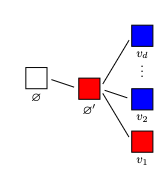
\includegraphics[width=0.1\textwidth]{frog_star.png}
            \end{tikzfigure}
            

                \item Even for values of $d$ as low as 5, the distribution of $U$ is extremely tedious to compute by hand. A naive computer algorithm gets stuck at around $d=30$. \edit{FC - I'll probably rewrite this bullet point.}
        \end{itemize}
        % \edit{EY - the stuff above might be a bit wordy. Feel free to cut it down. But I do feel like we should have some kind of broad overview.}

        \innerblock{hello}{hello}
    
}



\end{columns}
\end{document}